\section{Experiment Overview}

Below we summarize the three hardware parameters explored in this study, as well
as details of our per interrupt log collection tool.
%% \begin{figure}
%%   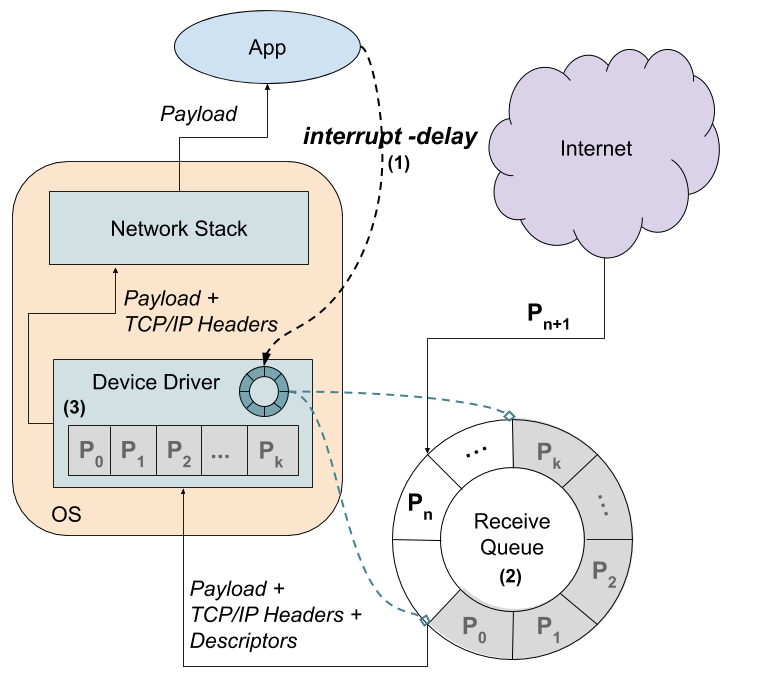
\includegraphics[width=7.7cm]{itr_figure.png}
%% \caption{As interrupt delay (1) is increased, the receive queue (2) buffers
%% more incoming packets as the NIC cannot fire new interrupts until the delay
%% value has been reached. Once the interrupt is fired, Linux's NAPI polling
%% mechanism kicks in and starts pulling in new packets (3) to be processed until
%% it either reaches its current work budget (calculated using existing jiffies)
%% or until there is no more data to be processed.}
%%   \label{fig:itr_figure}
%% \end{figure}

\subsection{Hardware Tuning Parameters}
Below, we discuss the three hardware parameters that are tuned statically in
this work:
\label{sec:knobs}
\begin{itemize}
\item \textbf{interrupt-delay}: Most modern NICs have a hardware feature to
control per receive interrupt rates.
The Intel 82599 datasheet~\cite{82599} defines a time-based interrupt
throttling mechanism which controls the time delay between packet reception and
the firing of an interrupt on the receiving core.
Its value can be set from a range between \texttt{0} and \texttt{1024}
$\micro$s in increments of \texttt{2} $\micro$s.
%Figure~\ref{fig:itr_figure} illustrates the interaction of interrupt delay
%values with the rest of systems software.
%The effect of setting a higher interrupt delay results in potential buffering
%of receive packets, thereby increasing packet processing efficiency at a
%potential cost to response time.

Linux's network device driver uses a dynamic algorithm that seeks to tune the
interrupt delay value such that it better reflects the current workload.
It achieves this by using data received from the previous interrupt about
packet counts and bytes per packet.
These values are then used to classify the current state of the workload (ex:
latency driven vs. bulk compute) and tune the interrupt delay accordingly based
off pre-computed theoretical maximum wire speeds.
%received from the last interrupt and classifies them broadly into a set of
%ranges that are pre-computed based off theoretical maximum wire speeds.
%This delay tuning is applied upon the next interrupt occurrence.
It is possible to disable this dynamic algorithm through the flip of a bit
inside the device driver. After flipping this bit, \textit{ethtool} can then be
used to set new interrupt delay values to statically fire at a fixed rate.
In our experiments, we take advantage of this ability by setting ITR delay values statically for different applications.
%device driver [REF] updates the interrupt delay value dynamically after every
%packet receive to a value based on the current traffic pattern. This value can
%also be fixed to a static value which results in interrupts being fired every X
%microseconds where X is a configurable value.


%To demonstrate its behavior, we instrumented a simple logging tool into the
%IXGBE device driver.
%Figure~\ref{fig:itr_delays} shows a small snapshot of its values while running
%a Memcached workload.
%Each marker represents a new \textit{ITR-Delay} value.
%In its current implementation, it can only seek values between the range of 2
%to 126 microseconds.
%The reason for this is that it was never designed towards a use case of
%aggressively delaying packet receive interrupts to take advantage of energy
%proportionality under stringent SLAs, which can potentially result in setting
%\textit{ITR-Delay} values in the hundreds of microseconds.

%It is also possible to disable this dynamic algorithm through the flip of a
%bit inside the device driver.
%This requires a rebuild of the driver module as it was not a configurable
%parameter.
%After flipping this bit, we can use Linux's \textit{ethtool} to set new
%interrupt delay values statically to fire every X microseconds, where X is a
%configurable value.


\item \textbf{RAPL}: Running Average Power Limit (RAPL)~\cite{intel_rapl} is a
power limiting feature on Intel processors.
In our experiments, we use the RAPL model segment registers (MSR) registers to
set explicit power limits up to a default max of \texttt{135} Watts (\watt) in
a single package on the processor. The processor used in our experiments
contain two packages. When applying power limits, care must be taken to ensure
there is a minimum RAPL value such that an application's continued execution
can be sustained in this limited power budget.
%Applications often depend on hardware components that in turn rely on a
%minimum power supply to continue running.
%Hence, when considering energy efficient compute, calculating minimum RAPL
%values that would sustain the execution of a particular workload becomes
%important.
From some initial experiments, we found that our class of applications
continued to execute correctly at a minimum RAPL limiting of around \texttt{55}
\watt. RAPL also provides the MSR\_PKG\_ENERGY\_STATUS register which allows
software to query the energy usage (Joules) of a specific package with a
minimum sample time of 1 milliseconds.
This is the main method with which our per-application energy consumption
results are gathered. Past researchers have also shown its efficiacy as a tool for reporting energy use~\cite{}.

\item \textbf{DVFS}: Intel power states (p-states) is another energy saving
feature on Intel processors.
It allows users to set specific p-states for individual cores.
A p-state is a combination of the clock frequency and voltage that a core is
operating on. Typically,  p-states are set dynamically according to current
processor load by a policy governor in Linux called Dynamic Voltage Frequency
Scaling (DVFS). DVFS can be disabled, thereby enabling setting static p-state
values by writing directly to the IA32\_PERF\_CTL register~\cite{intel_msr}.
A p-state is the combination of a core's clock frequency and its voltage at
some ratio, however, it is unclear how it exactly translates to real processor
frequency.
Normally, p-states are set dynamically according to current processor load by
a policy governor in Linux called Dynamic Voltage Frequency Scaling (DVFS).
In addition, DVFS can also be disabled which enables a user to set specific
p-state values by writing to the IA32\_PERF\_CTL register~\cite{intel_msr}.
From reading MSR\_PERF\_STATUS register~\cite{intel_msr}, we found the range of
DVFS values that a default Linux sets its processor into starts at a minimum
value of \texttt{0xC00} and up to a maximum of \texttt{0x1D00}. We use this
range in our study to tune processor p-states as another hardware knob.
\end{itemize}

\subsection{Per-interrupt Log Collection}
\label{sec:log_collect}
In order to better understand the interactions of ITR, DVFS, and
RAPL with a server that is under some load, we instrument \textit{fine-grained
per-interrupt} log collection in both Linux and libOS' network device
driver on the interrupt handling path.
We collect the following information for every interrupt fired: received and
transmitted bytes, received and transmitted descriptors, and the current
timestamp (via \texttt{rdtsc} instruction), and various sleep state statistics.
In addition, we instrument per-core performance monitoring counters (PMCs) to
collect a set of hardware statistics after every millisecond of elapsed time:
instructions, cycles, reference cycles, last-level cache misses, and energy
used (using the MSR\_PKG\_ENERGY\_STATUS register).
This set of statistics helps us to both take a detailed look at the per-core
behavior and acquire a global perspective on overall resource usage when
hardware is tuned in different ways.
%While this data provides a breadth of directions to reason about the results
%below, we discovered that it can be helpful to focus on subsets of data points
%for different workloads.
We ensured that the logging mechanism added minimal overhead to application
performance by using non-temporal store instructions to store the collected
statistics into an in-memory array.
%We found that using non-temporal store instructions had more of an impact on
%the performance of EbbRT versus that of Linux.
%We believe that this could be due to the fact that EbbRT was built to be an
%efficient library OS and hence its performance is more observably affected by
%additional logging.
%\subsubsection{Measurements}
%\label{sec:measures}
%\begin{itemize}
%       \item Throughput and Latency: Throughput is defined to be the
%time-average of total data transferred. It is measured in units of
%[bytes/second].
%         Latency is a measure of the delay between a request and the
%corresponding response. It is measured in [seconds]. Due to the stochastic
%nature of latency, we follow the convention of measuring the 99th percentile of
%the latency distribution for multiple requests.
%Depending on the workload, either throughput or latency is a direct measure of
%network %performance.
         %[Any notes about exact measurement process?]
       %\item Energy and Power
    %     [Note about Joule counter]
         
     %  \item Instructions, Cycles, Cache-Misses
	%\item Device Driver Statistics
	%\item Sleep States
%\end{itemize}


\section{Experimental Setup}

\label{sec:exp_setup}
\subsection{Hardware}
Our experimental cluster consists of a total of 7 nodes with a mix of 16 core
Intel(R) Xeon(R) CPU E5-2690 @ 2.90GHz and 12 core Intel(R) Xeon(R) CPU
E5-2630L v2 @ 2.40GHz processors and NICs with a mix of Solarflare
Communications SFC9120 10G Ethernet Controller and Intel Corporation 82599ES
10-Gigabit SFI/SFP+.
The nodes have a mix of 126 GB and 250 GB RAM configurations.
The node used to boot into baremetal library OS and Linux contains a 16 core
Intel(R) Xeon(R) CPU E5-2690 @ 2.90GHz, with 125 GB of RAM and an Intel
Corporation 82599ES 10-Gigabit SFI/SFP+ NIC.
We ensured that the processor for both Linux and the library OS was setup as
similarly as possible by carefully configuring both IA-32 Architectural MSRs
and processor specific MSRs (Table 35-2 and 35-18 in Intel's system
programmer's manual~\cite{intel_msr}).

\subsection{Linux}
In order to ensure a fair comparison between an application running in a single
purpose library OS versus a general purpose OS, we create a set of Linux
appliances for each of the applications (see Section~\ref{sec:apps}) we intend
to run.
Their base OS is Debian 10.4 and we use a custom compiled 5.5.17 kernel built
using a modified configuration file built for performance following suggestions
from previous work studied Linux core operation
costs~\cite{10.1145/3341301.3359640}.

These appliances are specially constructed to run a RAM-based filesystem and
contain only a small set of system libraries and kernel modules required to run
their constituent applications. In order to minimize system noise, we disable
hyperthreads and Turbo Boost features on all  processors and pin all
applications to physical cores in order to reduce potential background noise.
In addition, ~\textit{irqbalance} is disabled and packet receive interrupts are
affinitized to their respective cores.

%Describe details of configurations considered and various policies and
%mechanisms we know our workloads interact with.  Eg.  device driver, itr, napi,
%idle sleep states, etc. Also discuss what app software used.

\subsection{Library OS}
We ported an existing library OS written in C++ to baremetal by writing a
network device driver for the Intel 82599 NIC. The device driver totals over
3000 lines of code and interfaces with its multicore TCP/IP network stack.

Our library OS's NIC driver inherently does not have a dynamic policy for
updating interrupt-delay values, this is due to the fact that Linux's dynamic
interrupt-delay policy implementation relying on particular assumptions about
jiffies and NAPI polling budgets which the library OS does not.

%todo: JA this is wrong we do not fire an periodic interrupt to force processing
%.     The RCU garbage collector is not for the driving of event processing
As our library OS follows an event-driven model, whereby on each core, an
interrupt is fired after every static period of time to check a list for new
events to process; we implement a simple idling algorithm in this event loop by
adding \texttt{monitor} and \texttt{mwait} instructions in order to recommend
an idling core to go directly into the deepest sleep state prior to the
execution of a \texttt{halt} instruction. The sleep state value is inferred
from the \texttt{intel\_idle} function in Linux for our specific processor. The
library OS's idling policy is more simplistic compared to Linux, which consist
of multi-level sleep states dependent on the current system load.
We were careful to ensure that both EbbRT and Linux were configured similarly
in terms of NIC features: receive-side coalescing (RSC) disabled, direct-cache
injection (DCA) disabled, receive-side scaling (RSS) enabled to distribute
packets for multi-core processing, hardware checksum offloading enabled. We
also ensured the same values for parameters such as number of NIC transmit,
receive descriptors and write-back thresholds for packet transmissions.


\subsection{Applications}
\label{sec:apps}
In this study, we use the following set of applications in order to cover a
range of network workloads.
\begin{itemize}
\item \textbf{Netpipe}~\cite{snell1996netpipe} involves sending messages of the
same size between two systems for a fixed number of iterations in a single
connection. Both the client and the server are single-threaded. In both
systems, the 10 GB link is close to saturation after a message of size over 700
KB. We fix the iteration count at 5000 and show results for a range of message
sizes. The libOS uses a NetPIPE inspired reimplementation of its underlying protocol to take advantage of zero copying and run-to-completion model of the LibOS

\item \textbf{Nodejs}~\cite{nodejs} consists of of a single client thread and a
single server thread with a single connection between them. The server is
running a simple server written for nodejs using its builtin \texttt{http}
module that responds to each GET request with small static messages of size 148
bytes. A single client running the wrk~\cite{wrk} benchmark is used to place a
load on the nodejs server, we modified this workload generator in order to place a fixed
100K request limit.
%In contrast to netpipe, the workload is not fixed and performance is measured
%in requests-per-second once the benchmark has finished running. Further, a
%nodejs web server is computationally heavier than netpipe.

\item \textbf{Memcached}~\cite{mcd} is a multi-threaded application that runs
on all 16 cores of our server node.
The SLA objective in this application is to maintain a tail latency defined by
99\% of requests being processed in under 500 $\micro$s.
A client node running mutilate~\cite{mutilate} with no additional network load
is the main driver for controlling and monitoring the experiment.
It has two responsibilities: (1) it coordinates with five other mutilate agent
nodes in order to generate requests to the server and (2) measures tail latency
of all requests made.
All five agent nodes are 16-core
machines, each core creates 16 connections, for a total of 1280 connections
amongst 5 nodes. This setup is able to saturate the single 16 core server.
Mutilate is configured to pipeline up to four connections to further increase
its request rate.
We run a representative load from Facebook~\cite{workloadanalysisfacebook}
(ETC) which represents the highest capacity deployment. It uses 20 - 70 byte
keys and 1 byte to 1 KB values and contains 75\% GET requests.
	
\item \textbf{Memcached-silo}~\cite{mcdsilo} is an addition on top of the
normal memcached protocol used to reflect a more complex workload which
includes a combination of latency sensitive network traffic and compute and
memory intensive TPC-C style transaction processing.
Memcached-silo was developed by previous work done on building
scalable $\micro$s-scale in-memory compute servers~\cite{zygos},  and we ported it to the libOS.
The configuration and SLA of memcached-silo follows from that of memcached
(listed above). Given its computationally heavier nature, we only needed two
16-core server nodes at 16 connections per core to saturate our memcached-silo
server.
\end{itemize}

\subsection{Hardware Tuning Methodology}
\label{sec:hw_tuning}
We statically set ITR, DVFS, and RAPL values on the server node of
every application and collect per-interrupt log statistics on the same machine;
the range of values with which we vary these hardware parameters are listed in
Section~\ref{sec:knobs}.
It should be noted that for each application, we further reduce the sets of
values explored based on small experiments done a priori. Some of these are due
to ensuring that (1) increasing interrupt-delay and lowering DVFS processor
frequency does not bring about SLA violations for the memcached applications,
(2) lowering RAPL power limits does not cause the application and/or overall
system to crash, and (3) hardware configuration values encompass a wide range
and can be applied towards a specific workload, and (4) allows us to gather all
the results in a timely manner.

Below, we list the additional details of hardware tuning on a per-application
basis:
     
\begin{itemize}
\item \textbf{Netpipe}: Four representative message sizes of 64B, 8KB, 64KB,
and 512KB with a fixed round trip of 5000 iterations are selected. In addition,
as netpipe consists of the same binary running both as a client and a server,
we configured interrupt-delay to be the same in both client and server nodes.
For each message size and hardware configuration, we run the experiment 10
times to ensure statistical stability.
    
\item \textbf{Nodejs}: The wrk~\cite{wrk} benchmark is used to place a load on
the nodejs server with 100K requests. We only apply hardware configuration on the
server and rerun the experiment 10 times as well.
    
\item \textbf{Memcached}: Mutilate is used to generate three different
requests-per-second (QPS) rates of 200K, 400K and 600K for a fixed period of 30
seconds each. For each QPS rate, we run it across the three systems 5 times for
statistical stability.
    
\item \textbf{Memcached-silo}: Lower QPS rates of 50K, 100K, and 200K are
targeted here due to its increased computation load per request. Similarly, per
QPS rate is run on all three systems 5 times each.
\end{itemize}



%     \item The experiments are run for various ITR, DVFS, and RAPL settings.
%In the single threaded workloads, RAPL was fixed at the linux default value of
%135 \watt since we found it had minimal impact compared to ITR and DVFS on
%total time and total energy in both Linux and EbbRT. We hypothesize this is
%because RAPL power limiting is applied to an entire CPU package, therefore the
%power used in running a single threaded application was not heavy enough to
%warrant the power limiting features to come into play.
%     \item Each experiment can be described uniquely by the configuration
%tuple - (OS, MSG, ITR, DVFS).
%     \item Each configuration was run 5-10 times to measure statistical
%stability.
%     \item When the OS is Linux, we use three distinct configurations:
%        \begin{itemize}
%            \item Default - Both ITR and DVFS are changed according to the
%default Linux policy.
    
%            \item Tuned: DVFS -  ITR varies according to the default Linux
%policy while DVFS is fixed to a constant. The value reported in this column
%corresponds to the configuration (searched across DVFS values) that results in
%the smallest EDP. The smallest EDP and the corresponding Throughput for the
%same configuration are reported.
            
%            \item Tuned: DVFS + ITR + RAPL are fixed to constant values. As
%before, the smallest EDP (searched across ITR, DVFS, RAPL) is reported along
%with the corresponding performance value.
            
%        \end{itemize}
%    \item Since EbbRT does not implement dynamic policies for either ITR or
%DVFS. we use two distinct configurations:
%        \begin{itemize}
%            \item BaseLine - This column measures EDP and Throughput for the
%best Linux configuration found by tuning both ITR and DVFS. This is a direct
%comparison of the two OS structures.
            
%            \item Tuned - This column reports the smallest EDP (searched
%across ITR and DVFS) and the corresponding Throughput value.
            
 %       \end{itemize}

%\subsection{NetPipe}
%\label{sec:exp_app:netpipe}
%\begin{itemize}
%    \item We run the experiment with four message sizes (MSG) - 64B, 8KB,
%64KB, and 512KB on each of Linux and EbbRT. Each experiment involves
%transmitting packets of fixed size for 5000 round trips between two machines
%running the same operating system (OS). The total time taken (T) and the total
%energy consumed (E) are measured.

%    \item For each unique configuration, we measure the average EDP
%(Energy*Time) and average Throughput (MSG * 5000 / Time). The averages and
%standard deviations are across the runs for each configuration.

%    \item Table \ref{tab:netpipe_linux} lists both the EDP and Throughput
%values
        
%    \item Table \ref{tab:netpipe_ebbrt} lists both the EDP and Throughput
%values for the following cases when the OS is EbbRT  (columns 5 and 6 of table
%\ref{netpipe_linux}).

%\end{itemize}

%\subsection{NodeJS}
%\label{sec:exp_app:nodejs}
%\begin{enumerate}
%\item A simple web server written for nodejs using its builtin http module
%that responds to each GET request with small static messages totaling 148
%bytes, pinned to one core. A single client running wrk~\cite{wrk} benchmark to
%place a load for 30 seconds. Throughput is measured in requests/sec achieved
%once the benchmark is finished.
%\end{enumerate}

%\subsection{Memcached}
%\label{sec:exp_app:mcd}
%\begin{enumerate}
%\item 16 core memcached server=
%\item Given a static configuration listed above, we use \textit{mutilate} to
%generate loads at different request per second (RPS) rates, each for a constant
%period of time while collecting additional system metrics. In Linux,
%\textit{perf} is used to gather these metrics at a per second timeslice since
%the MSR\_PKG\_ENERGY\_STATUS for reporting CPU power usage has a limited wrap
%around time. EbbRT is able to collect the same metrics as Linux as it contains
%a inbuilt ~\textit{Perf} class which reads directly from Intel's PMC registers
%and a ~\textit{Rapl} class which reads from Intel's RAPL registers. In EbbRT,
%an event is triggered to fire every second in order to log the corresponding
%data.
%\end{enumerate}
\begin{table*}[htb]
\centering
\begin{tabular}{|c||l||l|l||l|l|}
\hline
\multirow{2}{*}{\begin{tabular}[c]{@{}c@{}}Workload \\ Configuration\end{tabular}} & \multicolumn{1}{c||}{Linux Default} & \multicolumn{2}{c||}{Linux Tuned}                                                                                                             & \multicolumn{2}{c|}{LibOS}                                                                                                                    \\ \cline{2-6} 
                                                                                   & Min                      & \begin{tabular}[c]{@{}l@{}}min (stdev)\\ (itr,dvfs,rapl)\end{tabular} & \begin{tabular}[c]{@{}l@{}}max(\#,stdev)\\ (itr,dvfs,rapl)\end{tabular} & \begin{tabular}[c]{@{}l@{}}min (\#,stdev) \\ (itr,dvfs,rapl)\end{tabular} & \begin{tabular}[c]{@{}l@{}}max(\#,stdev)\\ (itr,dvfs,rapl)\end{tabular} \\ \hline
Netpipe 64B                                                                       &            0.93                       &   0.48              &   12.87              &    0.28           &     11.78       \\ 
                                                                                  &                                       & (2,0x1500,*)      & (80,0x1b00,*) &   (6,0x1c00,*)  & (80,0x1a00,*)       \\ \hline

Netpipe 8KB                                                                       &           2.94                        &      2.06            &     17.06           &   1.02       &    11.82         \\ 
                                                                                  &                                       & (10,0x1400,*)      & (80,0x1d00,*)     &   (6,0x1600,*)   & (80,0x1a00,*)  \\ \hline

Netpipe 64KB                                                                      &           48.02                       &   19.8               &    98.38             &   9.41       &   30.61          \\ 
                                                                                  &                                       & (10,0x1400,*)      & (80,0x1b00,*)      &   (6,0xc00,*)    & (80,0x1700,*)  \\ \hline
                                                                                  
Netpipe 512KB                                                                     &           615.84                      &   492.3              &     774.95          &     409.82    &    617.85        \\ 
                                                                                  &                                       & (28,0xc00,*)       & (80,0x1d00,*)      &   (26,0xc00,*)   & (6,0x1d00,*)   \\ \hline \hline 
                                                                                  
NodeJS                                                                            &           2278.76                     &   1906.12            &    9058.46           &   1022.7     &    7016.15          \\ 
                                                                                  &                                       & (2,0x1d00,135)     & (80,0xd00,135)     &   (4,0x1900,135) & (80,0x1d00,55)  \\ \hline \hline
                                                                                  
Memcached 200k                                                                    &           138605.71                   & 120600.24            &    923324.152        & 70586.05           & 663224.2    \\ 
                                                                                  &                                       & (10,0x1300,55)     & (400,0x1d00,135)   &   (2,0xf00,135)  & (400,0x1d00,95)   \\ \hline
                                                                                  
Memcached 400k                                                                    &         220502.12                     &  183042.57        &   1045078.44      & 72121.42          &   727015.758      \\ 
                                                                                  &                                       & (10,0x1900,75)    & (400,0x1d00,95)   &   (2, 0xf00, 55)  & (400,0x1d00,55)   \\ \hline


Memcached 600k                                                                    &         360475.92                     &  280160.59        &   1207046.022      &  72528.39             &   824519.588   \\ 
                                                                                  &                                       & (30,0x1d00,135)    & (400,0x1d00,135)  &   (2, 0xf00, 55)  & (400,0x1d00,135)   \\ \hline \hline

MCD-Silo 50k                                                                       &                                    &                 &                &              &             \\ \hline
MCD-Silo 100k                                                                      &                                    &                 &                &              &             \\ \hline
MCD-Silo 200k                                                                      &                                    &                 &                &              &             \\ \hline  \hline
\end{tabular}
\caption{Energy Performance Product (EPP) Summary. Min and Max values indicate the smallest and largest EPP observed across the range of hardware parameters swept and the parameter settings for which this value was achieved.  The min EPP is a value on the system's best energy-performance curve.}
\label{table:eppsum}
\end{table*}
